\chapter{Podstawy teoretyczne}

\section{Rozpoznawanie emocji}

Rozpoznawanie emocji w dialogach koncentruje się na wydobyciu emocji przekazanej w rozmowie pomiędzy co najmniej dwoma rozmówcami. Problem ten stawia bardzo dużo wyzwań, takich jak obecność sarkazmu w rozmowie, przesunięcie emocji do kolejnych wypowiedzi tego samego rozmówcy oraz uchwycenie szerszego kontekstu pomiędzy wypowiedziami różnych osób. Dużym plusem w tej dziedzinie jest bardzo dobra dostępność do danych, które pochodzą z platform społecznościowych takich jak Facebook, Youtube, Reddit, Twitter \cite{poria2019emotion}. Poprzez łatwy dostęp do danych rozpoznawanie emocji w rozmowie staje się coraz bardziej popularne, a trudność tego problemu stwarza coraz to bardziej odległe granice co sprowadza się do wysokiego zainteresowania tą dziedziną przetwarzania języka naturalnego (ang. \textit{natural language processing - NLP}).

Bardzo ważnym elementem w rozpoznawaniu emocji jest możliwość zrozumienia danego przekazu w kontekście, od którego może zależeć rodzaj emocji. Szczególnie trudnym przypadkiem jest zrozumienie i zapamiętanie kontekstu w konwersacji, co jak pokazują autorzy artykułu na temat architektury głębokiego uczenia do rozpoznawania emocji w rozmowach tekstowych \cite{zhong2019knowledgeenriched}, może okazać się kluczowym czynnikiem skuteczności rozpoznawania emocji. Do uzyskania satysfakcjonujących wyników nie wystarczają tradycyjne metody uczenia maszynowego lub najbardziej podstawowe architektury sieci neuronowych \cite{kowsari2019text}. Modele te wykorzystują zaawansowane techniki architektury transformera (ang. \textit{the Transformer}) \cite{vaswani2017attention}, które korzystają z podejścia mającego na celu poprawę modelowania sekwencja do sekwencji (ang. \textit{Seq2Seq}) poprzez samoobserwację (ang. \textit{self-attention}) i kodowanie pozycji (ang. \textit{positional encoding}).

\section{Modele emocji}

Aby dobrze zrozumieć postawiony problem niezbędne będzie określenie czym są emocje. Wszyscy ludzie posiadają wrodzony zestaw podstawowych emocji, które można rozpoznać za pomocą gestów, czynów lub wypowiadanych słów. Możemy wyróżnić dyskretne emocje, aby móc odróżnić je od siebie. Istnieje kilka definicji różnych modeli emocji, jednym z nich jest model zaproponowany przez Paula Ekmana \cite{ekman1993facial}. Paul wraz ze współpracownikami stwierdzili, że istnieje sześć podstawowych emocji: gniew, obrzydzenie, strach, szczęście, smutek i zaskoczenie, a z każdą z tych emocji związane są jakieś cechy. Dzięki temu można wyrazić emocje w różnym stopniu a każda z nich jest zdefiniowana jako dyskretna kategoria, co pozwala na dość łatwą klasyfikację konkretnej emocji.

Kolejną definicję modelu emocji przedstawił Robert Plutchik, który podzielił emocje na osiem podstawowych typów, z których każdy ma drobniejsze podtypy pokrewne \cite{plutchik1982psychoevolutionary}, zaprezentowane na rysunku \ref{rys:plutchik_wheel} za pomocą koła emocji. Prezentuje on emocje jako koncentryczne kręgi, gdzie wewnętrzne części odpowiadają za podstawowe emocje a te zewnętrzne za bardziej złożone. Model ten jest dyskretny, lecz widać w nim pewne zależności i podobieństwa pomiędzy sąsiadującymi częściami koła emocji. Budowa ta wynika ze złożoności emocji i możliwości wyrażania ich intensywności.

\begin{figure}[t]
\centering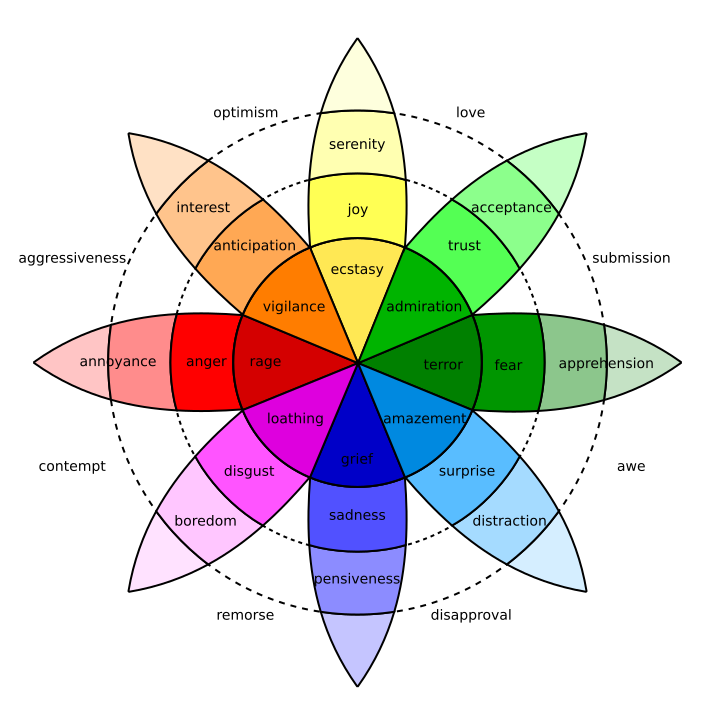
\includegraphics[width=10cm]{figures/plutchik-wheel.png}
\fcmfcaption{Koło emocji Plutchika \cite{plutchik1982psychoevolutionary}.}\label{rys:plutchik_wheel}
\end{figure}

Podsumowując wymienione modele emocji możemy wydzielić dwa główne typy: kategoryczne oraz wymiarowe. Modele wymiarowe mapują emocję w sposób ciągły na wektory. Modele kategoryczne klasyfikują emocję do konkretnej emocji dyskretnej, np. jednej z wybranego modelu emocji Ekmana lub Plutchika. Modele kategoryczne mają pewne wady. Jedną z nich jest brak możliwości opisania innych emocji oraz utrudnione opisywanie emocji złożonej z kilku różnych podtypów zdefiniowanych w dyskretnym modelu. Drugą wadą jest brak możliwości porównywania emocji, co umożliwiłby model wymiarowy, za pomocą porównywania dwóch wektorów. Wybór odpowiedniego modelu emocji nie jest łatwy, a jednocześnie jest bardzo ważnym elementem do późniejszej klasyfikacji emocji. Decydując się na kategoryczny typ emocji, z jednej strony mamy prosty model Ekmana który nie jest w stanie zamodelować złożonych emocji. Z drugiej strony w modelu Plutchika może być bardzo trudno rozróżnić drobnoziarniste emocje od siebie. Wybór ten należy zatem dokonać mając na uwadze wielkość oraz jakość zbioru danych.

\section{Głębokie uczenie}

W przetwarzaniu języka naturalnego z użyciem głębokich sieci neuronowych coraz częściej używane są techniki transferu wiedzy (ang. \textit{transfer learning}) oraz adaptacji domenowej. Model języka jest kluczowym elementem do zastosowania powyższych technik. Umożliwia on przewidzenie kontekstu w jakim dane słowo znajduje się w zdaniu i na tej podstawie umożliwia odkryć jego prawdziwy sens. Jest uważany za bardzo istotny element w dziedzinie \textit{NLP}, który stanowi podstawę do wszelkich zastosowań przetwarzania języka naturalnego. Najważniejsze jego cechy to zrozumienie długofalowych zależności i hierarchicznej struktury tekstu, a największe zalety to otwarte i wolne zasoby do jego stworzenia. Jest tworzony za pomocą nienadzorowanego procesu uczenia, który potrzebuje tylko korpusu nieoznakowanego tekstu.

Znakomitym przykładem użycia transferu wiedzy za pomocą wielokrotnego uczenia modelu języka jest metoda \textit{ULMFIT} \cite{howard2018universal} (ang. \textit{Universal Language Model Fine-tuning for Text Classification}, która może być zastosowana do każdego zadania w NLP. Zastosowane są w niej techniki, które są kluczowe dla dostrojenia modelu językowego. Używane są w niej 3 warstwy sieci neuronowej wykorzystującej komórki LSTM (ang. \textit{Long Short-Term Memory}), które w przeciwieństwie do standardowych komórek sieci neuronowych, posiadają połączenia zwrotne, umożliwiające zapamiętanie sąsiednich stanów w sieci. Dodatkowo zastosowana jest technika przerywania (ang. \textit{dropout}) niwelująca problem przeuczania. Cały etap nauki w metodzie \textit{ULMFIT} składa się z 3 etapów zaprezentowanych na rysunku \ref{rys:ulmfit}. Na początku następuje szkolenie wstępne modelu językowego na dowolnym korpusie, następnie dostrojenie modelu językowego na zadaniu docelowym i na końcu dostrojenie klasyfikatora na zadaniu docelowym. Dzięki zastosowaniu tych technik możliwe jest wyuczenie wstępne modelu języka na dowolnych danych, (np. korpus Wikipedii) a następnie wykorzystanie tego wstępnie wyuczonego modelu na zadaniu docelowym. Na podobnej zasadzie działają dzisiejsze najbardziej wyrafinowane architektury głębokich sieci neuronowych w zastosowaniu przetwarzania języka naturalnego nazywane aktualnym stanem techniki (ang. \textit{state of the art}).

\begin{figure}[t]
\centering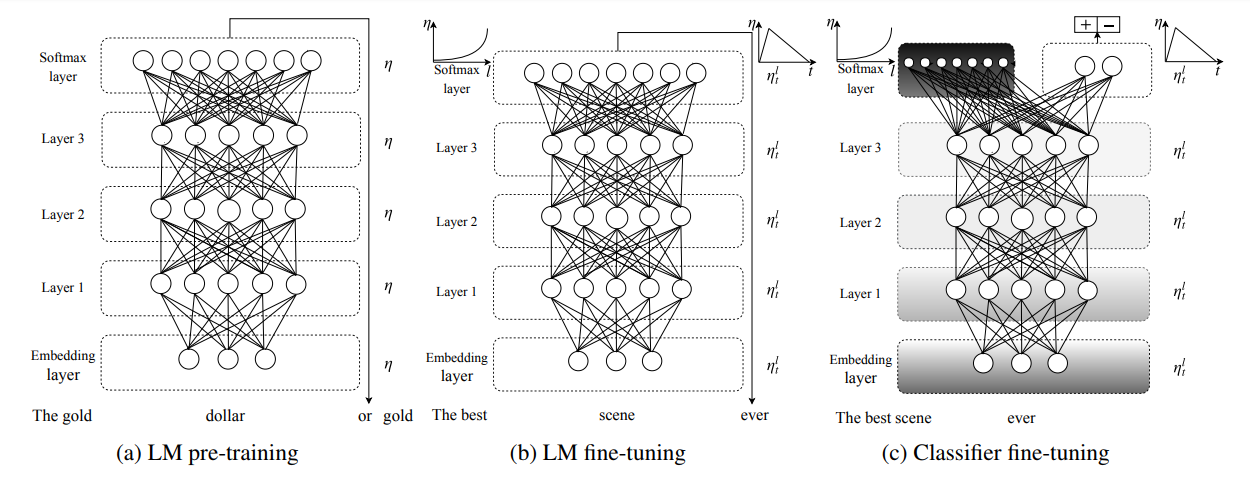
\includegraphics[width=\textwidth]{figures/ulmfit.png}
\fcmfcaption{3 etapy nauki modelu języka (ang. \textit{LM}) w metodzie ULMFIT \cite{howard2018universal}.}\label{rys:ulmfit}
\end{figure}